\documentclass[crop,tikz,convert=pdf2svg]{standalone}

% Tikz settings optimized for causal graphs.
\usetikzlibrary{shapes,decorations,arrows,calc,arrows.meta,fit,positioning}
\tikzset{
	-Latex,auto,node distance =2 cm and 2 cm,semithick ,
	state/.style ={ellipse, draw, minimum width = 0.7 cm},
	point/.style = {circle, draw, inner sep=0.04cm,fill,node contents={}},
	bidirected/.style={Latex-Latex,dashed},
	el/.style = {inner sep=2pt, align=left, sloped}
}

\begin{document}   

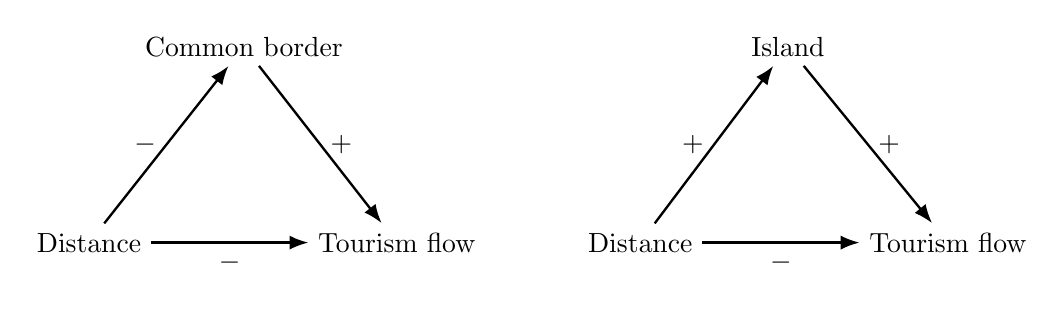
\begin{tikzpicture}

    \node (1) at (0,0) {Distance};
    \node (2) [right = of 1] {Tourism flow};
    \node (3) [above right =of 1,xshift=-2.2cm] {Common border};

    \path (1) [line width=0.03cm] edge node[below] {$-$} (2);
    \path (3) [line width=0.03cm] edge node[right] {$+$} (2);
    \path (1) [line width=0.03cm] edge node[left] {$-$}  (3);
    
    \node (1) at (7,0) {Distance};
    \node (2) [right = of 1] {Tourism flow};
    \node (3) [above right =of 1,xshift=-1.5cm] {Island};
    
    \path (1) [line width=0.03cm] edge node[below] {$-$} (2);
	\path (3) [line width=0.03cm] edge node[right] {$+$} (2);
	\path (1) [line width=0.03cm] edge node[left] {$+$}  (3);
    
\end{tikzpicture}
\end{document}
